\documentclass[a4paper,11pt]{book}
%\documentclass[a4paper,twoside,11pt,titlepage]{book}
\usepackage{listings}
\usepackage[utf8]{inputenc}
\usepackage[spanish]{babel}

% \usepackage[style=list, number=none]{glossary} %
%\usepackage{titlesec}
%\usepackage{pailatino}

%\decimalpoint
\usepackage{dcolumn}
\usepackage{float}
\newcolumntype{.}{D{.}{\esperiod}{-1}}
\makeatletter
%\addto\shorthandsspanish{\let\esperiod\es@period@code}
\makeatother


%\usepackage[chapter]{algorithm}
\RequirePackage{verbatim}
%\RequirePackage[Glenn]{fncychap}
\usepackage{fancyhdr}
\usepackage{graphicx}
\usepackage{afterpage}

\usepackage{longtable}

\usepackage[pdfborder={000}]{hyperref} %referencia

% ********************************************************************
% Re-usable information
% ********************************************************************
\newcommand{\myTitle}{Trabajo 3 - Evaluación Continua\xspace}
\newcommand{\myDegree}{MÁSTER EN INVESTIGACIÓN EN INGENIERÍA DE SOFTWARE Y
SISTEMAS INFORMÁTICOS\xspace}
\newcommand{\myName}{César Hugo Bárzano Cruz\xspace}
\newcommand{\myProf}{Nombre Apllido1 Apellido2 (tutor1)\xspace}
\newcommand{\myOtherProf}{Nombre Apllido1 Apellido2 (tutor2)\xspace}
%\newcommand{\mySupervisor}{Put name here\xspace}
\newcommand{\myFaculty}{ Universidad Nacional de Educación a Distancia\xspace}
\newcommand{\myFacultyShort}{UNED-Facultad de informática\xspace}
\newcommand{\myDepartment}{\xspace}
\newcommand{\myUni}{\protect{ Universidad Nacional de Educación a Distancia}\xspace}
\newcommand{\myLocation}{Madrid\xspace}
\newcommand{\myTime}{\today\xspace}
\newcommand{\myVersion}{Version 0.1\xspace}


\hypersetup{
pdfauthor = {\myName hugobarzano@gmail.com},
pdftitle = {\myTitle},
pdfsubject = {},
pdfkeywords = {},
pdfcreator = {LaTeX con el paquete TEXmaker},
pdfproducer = {pdflatex}
}

%\hyphenation{}


%\usepackage{doxygen/doxygen}
%\usepackage{pdfpages}
\usepackage{url}
\usepackage{colortbl,longtable}
\usepackage[stable]{footmisc}
%\usepackage{index}

%\makeindex
%\usepackage[style=long, cols=2,border=plain,toc=true,number=none]{glossary}
% \makeglossary

% Definición de comandos que me son tiles:
%\renewcommand{\indexname}{Índice alfabético}
%\renewcommand{\glossaryname}{Glosario}

\pagestyle{fancy}
\fancyhf{}
\fancyhead[LO]{\leftmark}
\fancyhead[RE]{\rightmark}
\fancyhead[RO,LE]{\textbf{\thepage}}
\renewcommand{\chaptermark}[1]{\markboth{\textbf{#1}}{}}
\renewcommand{\sectionmark}[1]{\markright{\textbf{\thesection. #1}}}

\setlength{\headheight}{1.5\headheight}

\newcommand{\HRule}{\rule{\linewidth}{0.5mm}}
%Definimos los tipos teorema, ejemplo y definición podremos usar estos tipos
%simplemente poniendo \begin{teorema} \end{teorema} ...
\newtheorem{teorema}{Teorema}[chapter]
\newtheorem{ejemplo}{Ejemplo}[chapter]
\newtheorem{definicion}{Definición}[chapter]

\definecolor{gray97}{gray}{.97}
\definecolor{gray75}{gray}{.75}
\definecolor{gray45}{gray}{.45}
\definecolor{gray30}{gray}{.94}

\lstset{ frame=Ltb,
     framerule=0.5pt,
     aboveskip=0.5cm,
     framextopmargin=3pt,
     framexbottommargin=3pt,
     framexleftmargin=0.1cm,
     framesep=0pt,
     rulesep=.4pt,
     backgroundcolor=\color{gray97},
     rulesepcolor=\color{black},
     %
     stringstyle=\ttfamily,
     showstringspaces = false,
     basicstyle=\scriptsize\ttfamily,
     commentstyle=\color{gray45},
     keywordstyle=\bfseries,
     %
     numbers=left,
     numbersep=6pt,
     numberstyle=\tiny,
     numberfirstline = false,
     breaklines=true,
   }

% minimizar fragmentado de listados
\lstnewenvironment{listing}[1][]
   {\lstset{#1}\pagebreak[0]}{\pagebreak[0]}

\lstdefinestyle{CodigoC}
   {
	basicstyle=\scriptsize,
	frame=single,
	language=C,
	numbers=left
   }
\lstdefinestyle{CodigoC++}
   {
	basicstyle=\small,
	frame=single,
	backgroundcolor=\color{gray30},
	language=C++,
	numbers=left
   }


\lstdefinestyle{Consola}
   {basicstyle=\scriptsize\bf\ttfamily,
    backgroundcolor=\color{gray30},
    frame=single,
    numbers=none
   }


\newcommand{\bigrule}{\titlerule[0.5mm]}


%Para conseguir que en las páginas en blanco no ponga cabecerass
\makeatletter
\def\clearpage{%
  \ifvmode
    \ifnum \@dbltopnum =\m@ne
      \ifdim \pagetotal <\topskip
        \hbox{}
      \fi
    \fi
  \fi
  \newpage
  \thispagestyle{empty}
  \write\m@ne{}
  \vbox{}
  \penalty -\@Mi
}
\makeatother

\usepackage{pdfpages}
\begin{document}
\begin{titlepage}
 
 
\newlength{\centeroffset}
\setlength{\centeroffset}{-0.5\oddsidemargin}
\addtolength{\centeroffset}{0.5\evensidemargin}
\thispagestyle{empty}

\noindent\hspace*{\centeroffset}\begin{minipage}{\textwidth}

\centering

\includegraphics[width=0.7\textwidth]{imagenes/Logo-uned.jpg}\\[1.1cm]


{\Huge\bfseries Máster Universitario En Investigación En Ingeniería De Software Y Sistemas Informáticos\\
}
\noindent\rule[-1ex]{\textwidth}{3pt}\\[3.5ex]
{\large\bfseries Generación Automática de Código}
\end{minipage}

\vspace{2.5cm}
\noindent\hspace*{\centeroffset}\begin{minipage}{\textwidth}
\centering

\textbf{Autor}\\ {César Hugo Bárzano Cruz}\\[2.5ex]


\includegraphics[width=0.3\textwidth]{imagenes/Logo-master.png}\\[0.1cm]
\textsc{Trabajo de Investigación}\\
\textsc{---}\\
2017/2018
\end{minipage}
%\addtolength{\textwidth}{\centeroffset}
%\vspace{\stretch{2}}
\end{titlepage}




%\frontmatter
\tableofcontents
\listoffigures
%\listoftables

%
%\mainmatter
%\setlength{\parskip}{5pt}

%\input{capitulos/01_Introduccion}


\chapter{Resumen}

En la actualidad, el desarrollo de aplicaciones web basadas en servicios ha marcado un antes y un despues, haciendo que los datos tomen un nuevo valor. La transformación digital es un hecho que esta cambiado el modo en que las empresas y usuarios interactuan con la información puesto que el acceso a los datos facilita la toma de decisiones, datos que hasta hace unos años no se pensaba que tendrían el valor social y económico que tienen hoy en día.

Es notable como la información y los canales de comunicacíon crecen día a día sadisfaciendo necesidades incubiertas que el usuario no conocia, automatizando procesos de negocio y mejorando tareas de gobierno.  

El desarrollo de aplicaciones web normalmente va asociado a procesos de desarrollo ágil donde se premia la alta disponibilidad, la rápida creación y la integración de nuevos servicios de información con los ya disponibles. Estas metodologias son responsables en su justa medida del rápido crecimiento de lo denominado WEB 2.0 o infraestructura de información distribuida a la cual, todos podemos acceder con los innumerables dispositivos que nos rodean. 

Estas metodologias, con aspectos muy beneficiosos para el ingeniería del software, tienen ciertas carencias con respecto a las metodologías de desarrollo tradicional. Si por un momento, dejamos de lado las tecnologías de la información y nos centramos en otros sectores  donde el software cumple un papel vital, como por ejemplo proyectos en el ambito espacial, defensa, automoción o aeronáutica, las lineas de desarrollo ágil son rechazadas por completo, puesto que el software resultante de estos proyectos ha sido validado y testeado durante largos años, siguiendo la metodología de desarrollo en V en la cual profundizaremos mas adelante. El desarrollo de estos proyectos conlleva la ejecución de lo denominado como "Plan de Validación" que si mismo es un proyecto de grandes proporciones que acompaña al proyecto principal durante todas sus etapas. El plan de validación de un proyecto establece el camino o manera en la que se valida el correcto funcionamiento del proyecto final, es decir, asegurar al cliente de que todos los requisitos planteados en fase de diseño se cumplen, produciendo así un sistema final fiable. 

El plan de validación en terminos de coste y tiempo tiene una proporciones considerables principalmente por que el proceso de refinamiento es lento, por lo que toman vital inportancia la automatización de pruebas y procedimiento, obteniendo una ganacia en hombre/tiempo significativa. Si quisieramos aplicar procedimientos similares al desarrollo de aplicaciones web basadas en metodologías agiles, seria necesario encontrar el termino medio entre un desarrollo ágil y un plan de validación que asegure el correcto funcionamiento de estos servicios de información. Debido a esto, el objetivo de esta investigación es el de intentar aplicar técnicas de validación tradicionales a procesos de desarrollo ágil, donde la generación automática de código desempeña un papel fundamental para la automatización de dichas pruebas. 

El resultado de esta investigación serán la generación automática de las pruebas necesarias para validar que aplicaciones de caracter web desarrolladas de manera ágil funcionan de la manera esperada, sin que dicho proceso de testeo suponga un pronblema en terminos de tiempo o dinero.  
 

\chapter{Introducción}

En los últimos años, la WEB 2.0 ha evolucionado de manera veloz debido a la gran demanda de infomación que tanto usuario como empresa han generado con el uso de las nuevas tecnologías. Esta demanda en ocasiones puede ocasionar ciertos problemas a la hora de ofrecer servicios de infomación ya que se disponibilizan servicios o versiones cuyo estado no es fiable, bajo el escudo de que los servicios de la información son de caracter volátil. Disponibilizar servicios no validados puede suponer una mala toma de decisiones pues el usuario medio asume la disponibilidad de estos o incluso la veracidad de la información proporcionada. 

El problema radica en que las metodologias de desarrollo para este tipo de servicios normalmente son de caracter ágil y los servicios expuestos normalmente no han superado un plan de validación adecuado ya que esto supone un incremento económico en el proceso de desarrollo y una notable dilatación en el tiempo de producción de nuevos releases debido a que la validación y verificación software mediante un enfoque tradicional es un proceso lento y pesado.

Para ello, con el foco en el desarrollo ágil de aplicaciones se va a plantear una solución a como los servicios de la información han de exponerse al mundo, garantizando que su resultado final es el esperado aplicando tecnicas de validación tradicional a los procesos de desarrollo ágil, siendo aquí donde la generación automática de código desempeñará un papel fundamental, ya que se intentará automatizar el proceso generativo del plan de validación de estos servicios. De esta manera, la solución final, verificará el desarrollo de aplicaciones sin incluir la dilatión en el tiempo que conlleva la ejecución de un plan de validación completo sobre un proyecto software.    

\chapter{El Problema}

En el desarrollo de servicios web y sus interfaces, normalmente mediante REST y SOAP, es muy común encontrar problemas relacionados con la perdida de servicio o la seguridad. Muchos de estos problemas son fruto de un desarrollo apresurado o puesta en producción de servicios de la información que no han pasado por etapas de revisión o certificación. Esto produce que los consumidores de estos servicios, normalmente otros servicios o frontales utilizados por cliente sufran fallos, ya que el canal o flujo de datos que alimenta todo la cadena no cumple lo esperado o las interfaces no son complaint con lo prometido a terceros. Estos problemas surgen a raíz de una mala validación de estos servicios. 

\subsection{Validación Software}

La validación\cite{v} software es un proceso de refinamiento en el que se garantiza el correcto funcionamiento del sistema validado, garantizando el correcto diseño e implementación de los requisitos planteados para el proyecto. Es un proceso largo y costoso con las dimensiones de un proyecto en si mismo donde se establece un plan de validación formado de campañas de verificación donde se establece la manera en la que se certifica el funcionamiento del software validado en cada una de las etapas del proyecto. La validación software normalmente sigue la metodología en V, donde a cada etapa del proyecto, le acompaña una etapa del plan de validación: 
\begin{figure}[H]  
\centering 
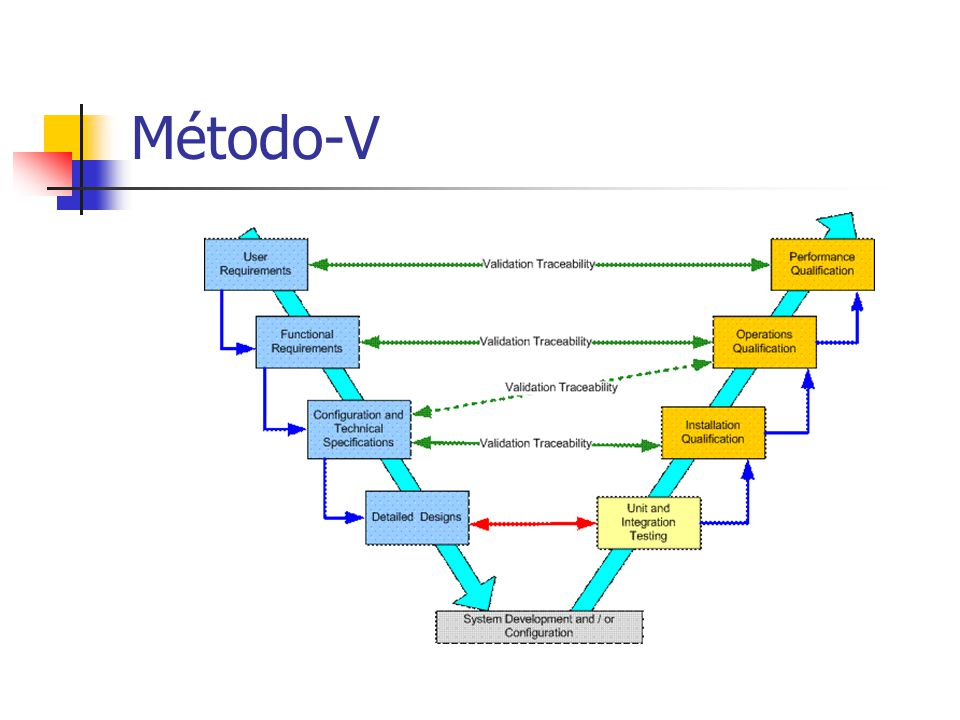
\includegraphics[scale=0.35]{imagenes/v.jpg}
\caption{ Método V }  
\end{figure} 

En terminos de tiempo y costes, este proceso es muy costoso por lo que se intenta automatizar en la medida de lo posible todas las tareas de testing asociadas a la etapa del desarrollo en la que el proyecto se encuentra.

El plan de validación en si, trata de establecer estas etapas del proyecto, definiendo los aspectos a cubrir en cada una de las entregas software establecidas por calendario. Cada entrega esta formada por una serie de casos de prueba o TestCases que aglutinan un conjunto de requisitos o funcionalidades a validar. Normalmente este conjunto es de alto nivel, por lo que los casos de prueba a su vez estan formados por una serie de TestSteps o pasos para validar cada uno de los requisitos de alto nivel definidos para el sistema. Cada TestSteps esta formado por uno o varios criterios PASS/FAIL. Esta cadena puede extenderse hacia arriba, tantos niveles como complejitud tenga el software que se intenta validar. Si trasladamos estas tecnicas al proceso de generación de servicios web, el coste en terminos de tiempo y dinere para el desarrollo ágil de servicios se vería altamente encarecido.  

\section{Tecnicas Usadas}

Actualmente, para solventar este tipo de problemas aplicados a los servicios de la información existen metodolgias como el test driven development o desarrollo basado en test donde primero se desarrollan los casos de prueba y despues el software necesario para pasar dichas pruebas. Tambien existen herramientas como Postman\cite{postman} para testear las interfaces expuestas a los frontales u otros servicios o SeleniumHQ\cite{selenium} para la automatización desde navegador. El problema de usar tecnologías como estas radica en la lentitud de las mismas, ya que apesar de ser muy potentes y perseguir la automatización, el tiempo de especificacion de lo que se quiere ejecutar es muy elevado, incluyendo restricciones propias que por contrato y base-line tecnológico imponen los diversoso proyectos, limitando las herramientas aceptadas para la validación de los mismos. 
\chapter{La Solución}

En vista de los problemas ocasionados por una mala validación de los servicios de información expuestos y debido a las carenciás que tienen las herramientas actuales para el testing de servicios web, se propone la creación de un generador de pruebas para las interfaces de ciertos servicios web con sus consumidores o aplicaciones cliente. 

\section{El Generador}

Se propone la implementación de un generador cuyas entradas sean ficheros de especificación para API-REST como RAML, JSON, XML y su salida sean los dintintos TestCases que se especifiquen como necesarios para validar el correcto funcionamiento del servicio web en cuestión. Dichos TestCases estaran formados por una serie de pasos o TestSteps con la especificación atómica que se ha de validar en ese paso, donde el resultado de la ejecución de este paso sea del criterio tipo pasa/no pasa. 

El generador resultante ha de entenderse como una herramienta propia para el desarrollo, ya que permitirá al desarrollador validar de forma rápida que el servicio en cuestión esta siendo construido de manera adecuada y que las interfaces expuestas efectivamente cumplen con lo deseado. 

\section{Tecnologías Utilizadas}

Como tecnología base, se ha decidido utilizar el lenguaje de programación GO\cite{go}, versión 1.10 debido a la eficiencia y facilidad que dicho lenguaje proporciona para el procesamiento de cadenas de caracteres. Como tecnología de salida, el generador es capaz de producir casos de prueba en bash\cite{bash} shell script. Se ha decido generar shell script debido a su alta eficiencia, ya que todo lo construido son sentencias interpretadas por el propio sistema operativo. Esto es altamente beneficioso a la hora de ejecutar grandes conjuntos de pruebas. Al generar código capaz de ser interpretado por el sistema operativo, no es necesaria la instalación de librerias de terceros o software adicional, lo cual es ideal para mantener la integridad de los entornos de desarrollo. Al tratarse de pruebas para las interfaces expuestas por los servicios de la información, si contamos con una máquina de pruebas con salida a internet capaz de consumir dichos servicios web, las pruebas tambien podria ser ejecutadas de manera remota y así obtener métricas sobre el estado de la red. 

El sistema operativo base sobre el que se han realizado las pruebas es Ubuntu\cite{ubuntu} 18.04 LTS atacando a una serie de servicios web que se ejecutan en el mismo sistema operativo pero dentro de contenedores o dockers. 

Adicionalmente para la confección de esta memoria se ha utilizado LaTEX con el paquete de librerías texlive-full y el editor texmaker. Los siguientes enlaces muestran como instalar y utilizar correctamente LaTEX, han sido utilizados como referencia para el presente documento. 

\begin{enumerate}
\item \href{http://milq.github.io/install-latex-ubuntu-debian/}{Instalar LaTeX}
\item \href{ http://minisconlatex.blogspot.com.es/}{Usar LaTeX}
\end{enumerate}
 
\section{Especificación de la Solución}

Al hablar de servicios web, es necesario tener en cuenta que estos hace uso del protocolo HTTP por lo que los códigos de estado devueltos por el protocolo son los que marcan el comportamiento de las peticiones atendidas por el servicio web. 

\begin{figure}[H]  
\centering 
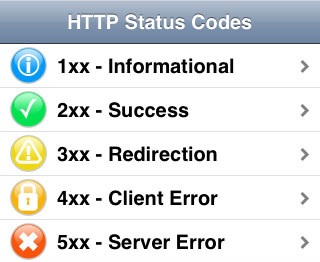
\includegraphics[scale=0.35]{imagenes/http.jpg}
\caption{ Método V }  
\end{figure}

Por ello, el generador recibirá como entrada un fichero de espedificación de api formado por entradas como la siguiente, donde establecer los atributos necesarios para validar que esta interfaz del servicio web es correcta. 

\begin{lstlisting}[language=python,caption={ Entrada Unitaria Configuración Generador }]
[{
  "name": "basic web app",
  "route": "/",
  "http_verb": "GET",
  "url": "http://localhost",
  "port":":8080",
  "body": "",
  "expected_code":"200"
}]

\end{lstlisting}

Para cada uno de estas entradas, el generador producirá el siguiente TestStep:  
\begin{lstlisting}[language=python,caption={ Test Step  }]
TestStep_0() {
echo "----- Test Step - 0 -----"
echo "TEST STEP - 0 "
echo "API NAME: basic web app"
echo "URL: http://localhost:8080/"

response_code=$(curl -XGET -i -k --write-out %{http_code} --output /dev/null http://localhost:8080/)

if [ $response_code = "200" ]; then
    echo "STEP - 0: PASS"
    echo "----- --- -----"
    return 0
else
  echo "STEP - 0: FAIL"
  return 1
fi
}
 \end{lstlisting}
 
 Con el conjunto de TestSteps que el generador produzca, se creará un TestCase como el que se muestra a continuación: 
 \begin{lstlisting}[language=python,caption={ Test Case  }]
 #!/usr/bin/env bash

echo
TestStep_0() {
echo "----- Test Step - 0 -----"
echo "TEST STEP - 0 "
echo "API NAME: basic web app"
echo "URL: http://localhost:8080/"

response_code=$(curl -XGET -i -k --write-out %{http_code} --output /dev/null http://localhost:8080/)

if [ $response_code = "200" ]; then
    echo "STEP - 0: PASS"
    echo "----- --- -----"
    return 0
else
  echo "STEP - 0: FAIL"
  return 1
fi
}
echo "----- --- -----"
echo

echo
TestStep_1() {
echo "----- Test Step - 1 -----"
echo "TEST STEP - 1 "
echo "API NAME: basic web app"
echo "URL: localhost:8080/users"

response_code=$(curl -XPOST -i -k --write-out %{http_code} --output /dev/null localhost:8080/users)

if [ $response_code = "" ]; then
    echo "STEP - 1: PASS"
    echo "----- --- -----"
    return 0
else
  echo "STEP - 1: FAIL"
  return 1
fi
}
echo "----- --- -----"
echo

TEST_PASS=0
TEST_FAIL=0
TOTAL_TEST=0
declare -a arr=("TestStep_0" "TestStep_1" )

for i in "${arr[@]}"
do
    if $i; then
        TEST_PASS=$((TEST_PASS+1));
    else
        TEST_FAIL=$((TEST_FAIL+1));
fi
done

echo
echo
echo "--- TEST CASE REPORT ---"
echo "TEST PASS: " $TEST_PASS
echo "TEST FAIL: " $TEST_FAIL
echo "TOTAL EXECUTED: " ${#arr[@]}
echo "--- --- --- --- --- ---"
 \end{lstlisting}

Este TestCase será el encargado de ejecutar todos los Test Steps, dando un informe del estado de la API, o APIS que se esten probando con la configuración de entrada.  
 
\section{Pruebas}

Con el Objetivo de mostrar la potencia del generador, se van a realizar una serie de ejecuciones de prueba para mostrar los posibles escenarios del generador. Para ello es necesario disponer de un servicio web sobre el que generar y ejecutar los casos de prueba generados.  En este caso, disponemos de un servicio de web basado contenedores ejecutalo localmente, los fuentes del servicio web usado para testear pueden encontrarse aquí
\href{DATARESTFUL}{https://github.com/hugobarzano/DataRestful}

\subsection*{TestCase1}

El primer caso de prueba, utilizará como configuracion un solo end-point de api y puede ser generado mediante \textbf{make generateTestCase1 }

 \begin{lstlisting}[language=python,caption={ TestCase1.json  }]
[{
  "name": "basic web app",
  "route": "/",
  "http_verb": "GET",
  "url": "http://localhost",
  "port":":8080",
  "body": "",
  "expected_code":"200"
}
]
\end{lstlisting}

El generador producirá la siguiente salida:
\begin{figure}[H]  
\centering 
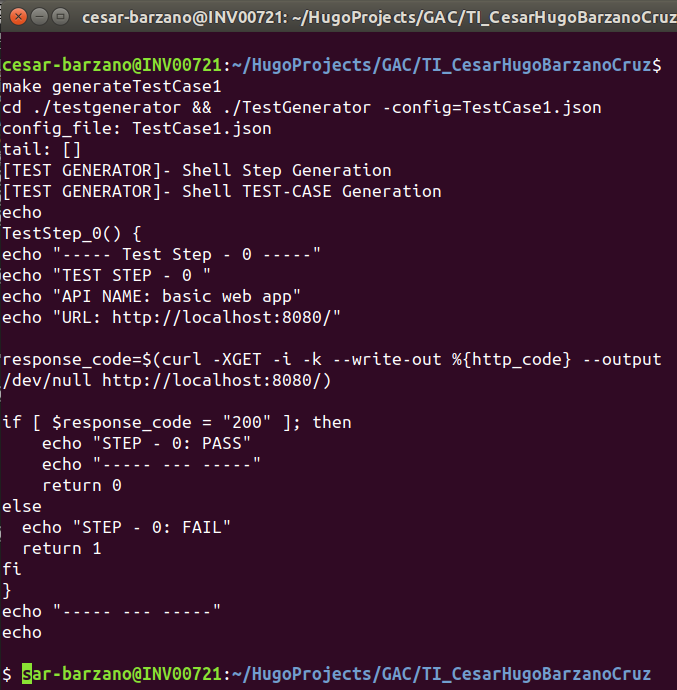
\includegraphics[scale=0.35]{imagenes/TestCase1_1.png}
\caption{ TestCase1 }  
\end{figure} 

Una vez generado el primer caso de prueba y con el servicio web corriendo, podemos ejecutarlo mediante \textbf{make runTestCase1} produciendo el siguiente resultado:

El generador producirá la siguiente salida:
\begin{figure}[H]  
\centering 
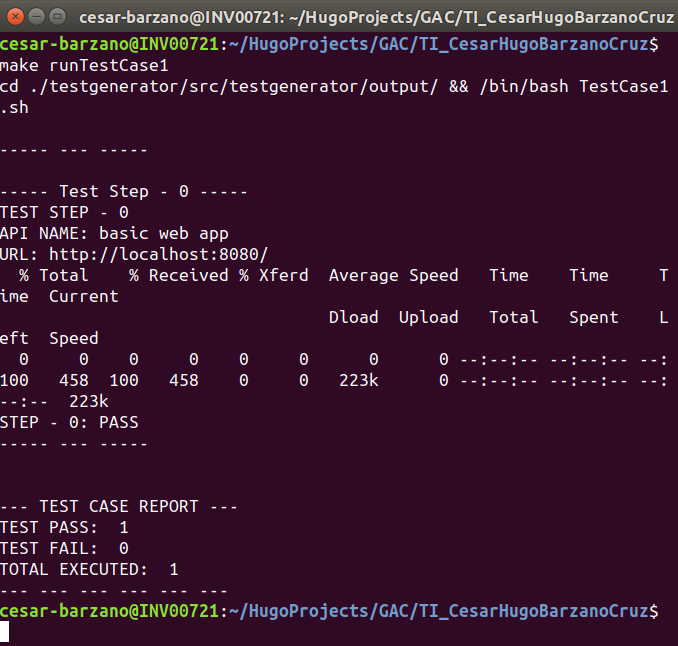
\includegraphics[scale=0.35]{imagenes/TestCase1_2.png}
\caption{ RUN TestCase1 }  
\end{figure} 


\subsection*{TestCase2}

El segundo caso de prueba, utilizará como configuracion un 2 end-point de api para disintos recursos y puede ser generado mediante \textbf{make generateTestCase2 }

 \begin{lstlisting}[language=python,caption={ TestCase2.json  }]
[{
  "name": "Datarestful - Index",
  "route": "/",
  "http_verb": "GET",
  "url": "http://localhost",
  "port":":8080",
  "body": "",
  "expected_code":"200"
},
  {
    "name": "Datarestful",
    "route": "/Services/",
    "http_verb": "GET",
    "url": "http://localhost",
    "port":":8080",
    "body": "",
    "expected_code":"200"
  }
]


\end{lstlisting}

Una vez generado el segundo caso de prueba y con el servicio web corriendo, podemos ejecutarlo mediante \textbf{make runTestCase2} produciendo el siguiente resultado:

\begin{figure}[H]  
\centering 
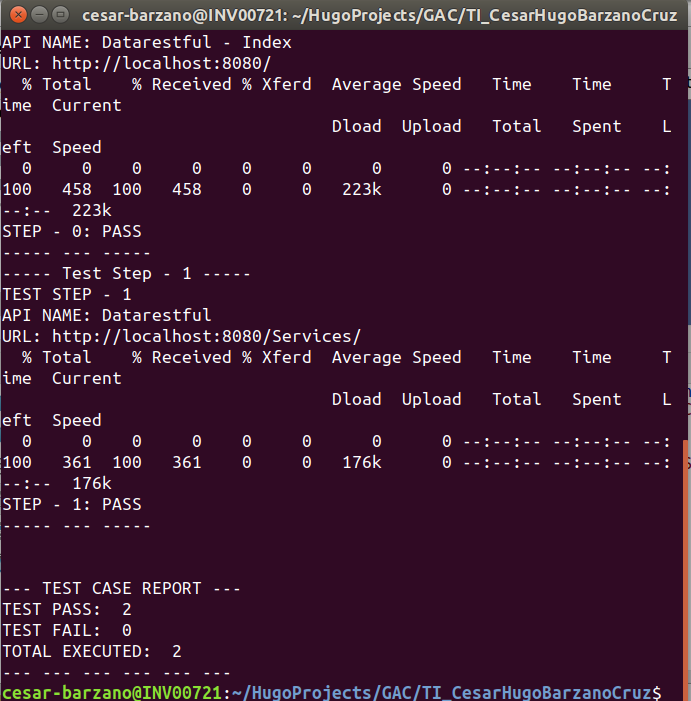
\includegraphics[scale=0.35]{imagenes/TestCase2_2.png}
\caption{ RUN TestCase2 }  
\end{figure} 


\subsection*{TestCase3}

El tercer caso de prueba, utilizará como configuracion un muchos end-point de api para disintos recursos y puede ser generado mediante \textbf{make generateTestCase3 }

 \begin{lstlisting}[language=python,caption={ TestCase3.json  }]
[{
  "name": "Datarestful - Index",
  "route": "/",
  "http_verb": "GET",
  "url": "http://localhost",
  "port":":8080",
  "body": "",
  "expected_code":"200"
},
  {
    "name": "Datarestful",
    "route": "/Services/",
    "http_verb": "GET",
    "url": "http://localhost",
    "port":":8080",
    "body": "",
    "expected_code":"200"
  },
  {
    "name": "Datarestful - Index",
    "route": "/",
    "http_verb": "GET",
    "url": "http://localhost",
    "port":":8080",
    "body": "",
    "expected_code":"200"
  },
  {
    "name": "Datarestful",
    "route": "/Services/",
    "http_verb": "GET",
    "url": "http://localhost",
    "port":":8080",
    "body": "",
    "expected_code":"200"
  },{
  "name": "Datarestful - Index",
  "route": "/",
  "http_verb": "GET",
  "url": "http://localhost",
  "port":":8080",
  "body": "",
  "expected_code":"200"
},
  {
    "name": "Datarestful",
    "route": "/Services/",
    "http_verb": "GET",
    "url": "http://localhost",
    "port":":8080",
    "body": "",
    "expected_code":"200"
  },{
  "name": "Datarestful - Index",
  "route": "/",
  "http_verb": "GET",
  "url": "http://localhost",
  "port":":8080",
  "body": "",
  "expected_code":"200"
},
  {
    "name": "Datarestful",
    "route": "/Services/",
    "http_verb": "GET",
    "url": "http://localhost",
    "port":":8080",
    "body": "",
    "expected_code":"200"
  }
]




\end{lstlisting}

Una vez generado el tercer caso de prueba usando \textbf{make generateTestCase3} y con el servicio web corriendo, podemos ejecutarlo mediante \textbf{make runTestCase3}. Al tratarse de 7 end-points de api, lo  generado y ejecutado mediante make es: 

\begin{lstlisting}[language=python,caption={ TestCase3.sh  }]
#!/usr/bin/env bash

echo
TestStep_0() {
echo "----- Test Step - 0 -----"
echo "TEST STEP - 0 "
echo "API NAME: Datarestful - Index"
echo "URL: http://localhost:8080/"

response_code=$(curl -XGET -i -k --write-out %{http_code} --output /dev/null http://localhost:8080/)

if [ $response_code = "200" ]; then
    echo "STEP - 0: PASS"
    echo "----- --- -----"
    return 0
else
  echo "STEP - 0: FAIL"
  return 1
fi
}
echo "----- --- -----"
echo

echo
TestStep_1() {
echo "----- Test Step - 1 -----"
echo "TEST STEP - 1 "
echo "API NAME: Datarestful"
echo "URL: http://localhost:8080/Services/"

response_code=$(curl -XGET -i -k --write-out %{http_code} --output /dev/null http://localhost:8080/Services/)

if [ $response_code = "200" ]; then
    echo "STEP - 1: PASS"
    echo "----- --- -----"
    return 0
else
  echo "STEP - 1: FAIL"
  return 1
fi
}
echo "----- --- -----"
echo

echo
TestStep_2() {
echo "----- Test Step - 2 -----"
echo "TEST STEP - 2 "
echo "API NAME: Datarestful - Index"
echo "URL: http://localhost:8080/"

response_code=$(curl -XGET -i -k --write-out %{http_code} --output /dev/null http://localhost:8080/)

if [ $response_code = "200" ]; then
    echo "STEP - 2: PASS"
    echo "----- --- -----"
    return 0
else
  echo "STEP - 2: FAIL"
  return 1
fi
}
echo "----- --- -----"
echo

echo
TestStep_3() {
echo "----- Test Step - 3 -----"
echo "TEST STEP - 3 "
echo "API NAME: Datarestful"
echo "URL: http://localhost:8080/Services/"

response_code=$(curl -XGET -i -k --write-out %{http_code} --output /dev/null http://localhost:8080/Services/)

if [ $response_code = "200" ]; then
    echo "STEP - 3: PASS"
    echo "----- --- -----"
    return 0
else
  echo "STEP - 3: FAIL"
  return 1
fi
}
echo "----- --- -----"
echo

echo
TestStep_4() {
echo "----- Test Step - 4 -----"
echo "TEST STEP - 4 "
echo "API NAME: Datarestful - Index"
echo "URL: http://localhost:8080/"

response_code=$(curl -XGET -i -k --write-out %{http_code} --output /dev/null http://localhost:8080/)

if [ $response_code = "200" ]; then
    echo "STEP - 4: PASS"
    echo "----- --- -----"
    return 0
else
  echo "STEP - 4: FAIL"
  return 1
fi
}
echo "----- --- -----"
echo

echo
TestStep_5() {
echo "----- Test Step - 5 -----"
echo "TEST STEP - 5 "
echo "API NAME: Datarestful"
echo "URL: http://localhost:8080/Services/"

response_code=$(curl -XGET -i -k --write-out %{http_code} --output /dev/null http://localhost:8080/Services/)

if [ $response_code = "200" ]; then
    echo "STEP - 5: PASS"
    echo "----- --- -----"
    return 0
else
  echo "STEP - 5: FAIL"
  return 1
fi
}
echo "----- --- -----"
echo

echo
TestStep_6() {
echo "----- Test Step - 6 -----"
echo "TEST STEP - 6 "
echo "API NAME: Datarestful - Index"
echo "URL: http://localhost:8080/"

response_code=$(curl -XGET -i -k --write-out %{http_code} --output /dev/null http://localhost:8080/)

if [ $response_code = "200" ]; then
    echo "STEP - 6: PASS"
    echo "----- --- -----"
    return 0
else
  echo "STEP - 6: FAIL"
  return 1
fi
}
echo "----- --- -----"
echo

echo
TestStep_7() {
echo "----- Test Step - 7 -----"
echo "TEST STEP - 7 "
echo "API NAME: Datarestful"
echo "URL: http://localhost:8080/Services/"

response_code=$(curl -XGET -i -k --write-out %{http_code} --output /dev/null http://localhost:8080/Services/)

if [ $response_code = "200" ]; then
    echo "STEP - 7: PASS"
    echo "----- --- -----"
    return 0
else
  echo "STEP - 7: FAIL"
  return 1
fi
}
echo "----- --- -----"
echo

TEST_PASS=0
TEST_FAIL=0
TOTAL_TEST=0

declare -a arr=("TestStep_0" "TestStep_1" "TestStep_2" "TestStep_3" "TestStep_4" "TestStep_5" "TestStep_6" "TestStep_7" )

for i in "${arr[@]}"
do
    if $i; then
        TEST_PASS=$((TEST_PASS+1));
    else
        TEST_FAIL=$((TEST_FAIL+1));
fi
done

echo
echo

echo "--- TEST CASE REPORT ---"
echo "TEST PASS: " $TEST_PASS
echo "TEST FAIL: " $TEST_FAIL
echo "TOTAL EXECUTED: " ${#arr[@]}
echo "--- --- --- --- --- ---"

\end{lstlisting}


\chapter{Entrega}
En este capítulo se detallan cada uno de los ficheros/directorios que forman parte de la entrega. 

\section{Generador}
El generador propuesto por el enunciado se compone de una serie de paquetes GO alojados dentro de testgenerator/src. El generador ha sido desarrollado sobre Ubuntu.18 y hace uso de la versión Go 1.10 pero al ser un lenguaje compilado, podemos elegir entre ejecutar el código fuente ( necesario tener GO instalado en el sistema o utilizar el ejecutable generado con la compilación.  

\section{Makefile}
El fichero ''makefile'' establece las distintas ejecuciones de pruebas para el generador.
 

\section{TI\_CesarHugoBarzanoCruz.pdf}
Memoría de la práctica, referencia a este documento en si mismo, alojado en el directorio raíz de la entrega. 

\section{Directorio DOC}
Directorio donde se almacenan todos los fuentes usados para generar esta documentación utilizando LaTEX. Incluye tambien las imagenes usadas en la memoria. 

\section{Directorio src/testgenerator/input}
Directorio donde se almacenan todos los ficheros usados como configuracion para el generador.

\section{Directorio src/testgenerator/output}
Directorio donde se almacenan todos los ficheros resultados de la ejecución de la pruebas. 

 

\begin{thebibliography}{aaaa}

%intro

\bibitem[1]{go} \textsc{GO},
\textit{The GO Programming Language}
\url{https://golang.org/} 


\bibitem[2]{ubuntu} \textsc{Ubuntu},
\textit{Ubuntu 18 TLS}
\url{https://www.ubuntu.com/} 

%Desarrollo

\bibitem[3]{bash} \textsc{BASH},
\textit{Shell BASH}
\url{https://linux.die.net/man/1/bash} 


\bibitem[4]{v} \textsc{Validation Plan},
\textit{Ofni Systems}
\url{http://www.ofnisystems.com/services/validation/validation-plans/} 

\bibitem[5]{postman} \textsc{Postman},
\textit{POSTMAN API DEVELOPMENT}
\url{https://www.getpostman.com/} 

\bibitem[4]{selenium} \textsc{Selenium},
\textit{Selemium Browser Automation}
\url{https://www.seleniumhq.org/} 

\end{thebibliography}
 

\chapter{Anexo}

\section{makefile}
\begin{lstlisting}[language=python,caption={makefile }]
#Makefile

install:
	sh ./install.sh

build:
	go build generadorP3.go

generateTestCase1:
	cd ./testgenerator && ./TestGenerator -config=TestCase1.json
runTestCase1:
	cd ./testgenerator/src/testgenerator/output/ && /bin/bash TestCase1.sh 
generateTestCase2:
	cd ./testgenerator && ./TestGenerator -config=TestCase2.json
runTestCase2:
	cd ./testgenerator/src/testgenerator/output/ && /bin/bash TestCase2.sh 
generateTestCase3:
	cd ./testgenerator && ./TestGenerator -config=TestCase3.json
runTestCase3:
	cd ./testgenerator/src/testgenerator/output/ && /bin/bash TestCase3.sh 


\end{lstlisting}



%
%
%%\nocite{*}
%\bibliography{bibliografia/bibliografia}\addcontentsline{toc}{chapter}{Bibliografía}
%\bibliographystyle{miunsrturl}
%
%\appendix

%\input{apendices/manual_usuario/manual_usuario}
%%\input{apendices/paper/paper}
%\input{glosario/entradas_glosario}
% \addcontentsline{toc}{chapter}{Glosario}
% \printglossary

\thispagestyle{empty}

\end{document}
